% Copyright 2023 Kieran W Harvie. All rights reserved.
\documentclass[12pt]{report}

\usepackage{amsmath}
\usepackage{hyperref}
\usepackage{amssymb}
\usepackage{tikz}
 
\usepackage[OT2,T1]{fontenc}

\title{Math Notes}
\date{Copyright \textcopyright  \today. All Rights Reserved.}
\author{Kieran Harvie}

\DeclareSymbolFont{cyrletters}{OT2}{wncyr}{m}{n}

\DeclareMathOperator{\sinc}{sinc}
\DeclareMathOperator{\Ai}{Ai}
\DeclareMathSymbol{\Sha}{\mathalpha}{cyrletters}{"58}
\DeclareMathOperator{\cl}{cl}
\DeclareMathOperator{\im}{Im}
\DeclareMathOperator{\rect}{rect}
\DeclareMathOperator{\sgn}{sgn}
\DeclareMathOperator{\XOR}{ XOR }
\DeclareMathOperator{\E}{\mathbb{E}}

\begin{document}
\maketitle
\tableofcontents

% Copyright 2023 Kieran W Harvie. All rights reserved.

\section{Mean and Variance, and the arbitrariness thereof}
For some time I have wondered about the arbitrariness around the mean and variance.
For example why the arithmetic mean instead of the geometric or root-mean-squared?
And why square root the variance to give the standard deviation?

Well the strictness of Markov's and Chebyshev's might provide a reason.
Both rely of the conditional expected value, so just to reiterate:
\[E[X | X \geq a] \geq a \]
Since everything $X$ can be is greater then $a$ it's expected value must be greater than $a$. 
Notice the strictness of the inequality, this will be used to make the following inequalities much stricter.

\subsection*{Markov}
\begin{equation*}
\begin{aligned}
	\mu =& E[X]\\
	=& P(X \leq a)E[X|X \leq a] + P(X \geq a)E[X|X \geq a] \\ 
	\geq& 0\cdot E[X|X \leq a] + P(X \geq a)a \\ 
	\frac{\mu}{a}\geq& P(X \geq a) \\
\end{aligned}
\end{equation*}
% What if we move zero around?
% try Y = m X+c and see what happens.

\subsection*{Chebyshev}
\begin{equation*}
\begin{aligned}
	& E[(X-a)^2] \\
	=&P(|X-a| \leq b)E[(X-a)^2 | |X-a| \leq b] + P(|X-a| > b)E[(X-a)^2 | |X-a| > b]\\
\end{aligned}
\end{equation*}

\subsection*{A General Relation}
Assume:
\[f(S') \geq 0,\quad g(S) \geq 0\]
Then through:
\begin{equation*}
\begin{aligned}
	E[f(X)] =& P(X \in S)E[f(X) | X \in S] + P(X \in S' )E[f(X) | X \in S']\\
\end{aligned}
\end{equation*}
We have:
\begin{equation*}
\begin{aligned}
	1 - \frac{E[g(X)]}{E[g(X) | X \in S']} \leq P[X \in S] \leq \frac{E[f(X)]}{E[f(X) | X \in S]}\\
\end{aligned}
\end{equation*}
With dual equality if:
\[f = 1_S,\quad g = 1_{S'}\]

\subsection*{Covariance}
Lets try to find the lest squares regression between $X$ and $Y$ such that:
\[E[X] = E[Y] = 0, E[X^2] = E[Y^2] = 1\]
Since the expected values are both zero the line is through the origin
\begin{equation*}
\begin{aligned}
	\sum_{n}(mx_n+c-y_n)^2 =& nE[(mX+c-Y)^2] \\
	=& n \bigg(E[m^2X^2]+E[c^2]+E[Y^2]+E[2cmX]+E[-2mXY]+E[-2cY]\bigg)\\
	=& n(m^2+c^2+1-2mE[XY])\\
\end{aligned}
\end{equation*}
Trying to minimize this value by our selection of trivially gets:
\[c = 0,\quad m = E[XY]\]
Just expanding the definitions gives:
\[COV[X,Y] = E[(X-E[X])(Y-E[Y])] = E[XY] = m\]
Hence the covariance can `naturally' be interpreted and the first order function between the valuables.

\[E[f(X)] \approx E[f_0 + f_1X + f_2X^2/2] = f_0 + \mu f_1 + \sigma^2f_2/2\]
\[E[f(X)] \approx E[f(\mu) + (X-\mu)f'(\mu) + (X-\mu)^2/2f''(\mu)] = f(\mu) + \frac{f''(\mu)}{2}\sigma^2\]

% Consider a mention of Bessel's correction and the sum((x-(mu+a)^2) = sigma^2+a^2, general relation (square through AM-GM inequality)

% Copyright 2023 Kieran W Harvie. All rights reserved.

\section{Interest Identities}
Let $P$ be the principle invested at a rate of $r$.
Consider four different investment scenarios:
\begin{itemize}
	\item Not invested: $P_0 = P$.
	\item Fully Invested at the beginning, one instalment at the end:
		\[P_1 = (1+r)P\]
	\item Continuously invested, continuous installments:
		\[P_2 = \lim_{n\rightarrow\infty}\sum_{k=0}^n\frac{P}{n}\left(1+\frac{r}{n}\right)^k = \frac{\exp(r)-1}{r}P\]
	\item Fully Invested at the beginning, continuous instalments: 
		\[P_3 = \lim_{n\rightarrow \infty}P\left(1+\frac{r}{n}\right)^n = \exp(x)P\]
\end{itemize}

Interestingly the relative size of $P_2$ and $P_1$ depend on $r$.
$P_1$ starts on $P_2$ but switches as $r$ increases.\\

$P_3$ is always the best, the proof for $P_1$ and $P_0$ are obvious.
$P_3 > P_2$ follows from:
\[0 < \int_0^rt\exp(t)\,dt = \big[(t-1)\exp(t)\big]_0^r = (r-1)\exp(r)+1\] \\

The following interesting identities hold:
\[P_3 = rP_2+P_0\]
\[P_3-P = r(P_2-P) + (P_1-P)\]
The breaks first neatly breaks $P_3$ into a nice linear sum.
The second does similar for the profit of the investment, total yield minus principle.

% Copyright 2023 Kieran W Harvie. All rights reserved.

\section{Discontinuities in a Non-decreasing Function}

Let $f$ be a non-decreasing function.

Define the jump function $J$ as:
\[ J(x) = \inf\{f(t) | t > x\} - \sup\{f(t) | t < x\}\]

This function is well defined since the sets are appropriately bound by $f(x)$. And it is clear that $J(d) \neq 0$ iff $d$  is a discontinuity and that $J$ is non-negative.
\\

Let $U = (x_0,x_1)$. For $d_n \in U$ with $n < m \Rightarrow d_n < d_m$ we have:
\[f(x_1)-f(x_0) \geq \sum_{k}J(d_k)\]

Proof:
\begin{equation*}
\begin{aligned}
	&\sum_{k}J(d_k) \\
	=& \inf\{f(t) | t > d_n\} - \sup\{f(t) | t < d_0\} + \sum_k\big[\inf\{f(t) | t > d_{k-1}\} - \sup\{f(t) | t < d_k\}\big] \\
	\leq & f(d_n)-f(d_0) + \sum_k\big[f(d_{k-1})-f(d_k)\big] \\
	\leq & f(d_n)-f(d_0)\\
	\leq & f(x_n)-f(x_0)\\
\end{aligned}
\end{equation*}

Let $ S_n = \{d \in U | J(d) > \frac{1}{n}(f(x_1)-f(x_0)) \}$
From the previous inequality there are at most $n$ elements in $S_n$.
Hence:
\[\{d\in U | J(d) > 0\} = \bigcup_{n}\left\{d \in U | J(d) > \frac{1}{n}(f(x_1)-f(x_0))\right\}\]
Is countable, hence the number of discontinuities of $f$ on $U$ is countable.
\\

By corollary the discontinuities of a non-decreasing function on $\mathbb{R}$ are countable:

Let $f$ be a non-decreasing function on $\mathbb{R}$.
Let $X_n = (n-1,n+1)$, clearly $\mathbb{R} = \bigcup_{n}X_n$\footnote{Having them overlap simplify the proof by avoiding literal edge-cases.}.
Assume $f$ has an uncountable number of discontinuities then at least one $X_n$ contains uncountable discontinuities.
Otherwise there would be a countable set of countable sets of discontinuities, making them countable.
But $f$ being non-decreasing function and having an uncountable number of discontinuities in $X_n$ is a contradiction.

% Copyright 2023 Kieran W Harvie. All rights reserved.

\section{Integrals and Symmetry}

\subsection{Domain Symmetry} 
Let $U$ be a subset of $\mathbb{R}^n$ and let $\phi: U \rightarrow U$ be a function such that:
\begin{equation*}
\begin{aligned}
	\phi(U) &= U \\
	|\det\phi'(\mathbf{u})| &= 1 \\
\end{aligned}
\end{equation*}
Basically $\phi$ is a linear permutation\footnote{
	Note that $\phi$ being a permutation requires that if the magnitude of the determinate is constant it must be unity, this can be seen by setting $f$ to a constant.
}
on $U$, this is a symmetry in the most direct sense.
We obtain the following:
\\
\begin{equation*}
\begin{aligned}
	\int_{U}f(\mathbf{v})\,d\mathbf{v} =& \int_{\phi(U)}f(\mathbf{v})\,d\mathbf{v} \\
	=& \int_Uf(\phi(\mathbf{u}))|\det\phi'(\mathbf{u})|\,d\mathbf{u} \\
	=& \int_Uf(\phi(\mathbf{u}))\,d\mathbf{u} \\
\end{aligned}
\end{equation*}
\\

In particular we get:
\[0=\int_{U}\big(f(\mathbf{u})-f(\phi(\mathbf{u}))\big)\,d\mathbf{u}\]

This integral is important since a function can be split into a vanishing and non-vanishing part:
\begin{equation*}
\begin{aligned}
	f(\mathbf{u}) =& \frac{1}{2}\big(f(\mathbf{u})+f(\phi(\mathbf{u}))+\frac{1}{2}\big(f(\mathbf{u})-f(\phi(\mathbf{u}))\big) \\
	\int_Uf(\mathbf{u})\,d\mathbf{u} =& \frac{1}{2}\int_U\big(f(\mathbf{u})+f(\phi(\mathbf{u}))\,d\mathbf{u}+\frac{1}{2}\int_U\big(f(\mathbf{u})-f(\phi(\mathbf{u}))\big)\,d\mathbf{u} \\
	=& \frac{1}{2}\int_U\big(f(\mathbf{u})+f(\phi(\mathbf{u}))\,d\mathbf{u}\\
\end{aligned}
\end{equation*}
\\

For example, consider the classic odd function on an integral centered at $0$.
\[\phi(x) = -x \]
\[U = [-1,1]\]

We get the familiar:
\[\int_{-1}^{1}f(x)\,dx = \frac{1}{2}\int_{-1}^{1}\big(f(x)+f(-x)\big)\,dx\]
\\

The utility of this relation can be seen by applying it to the basis of a class of function.
Let $V = \langle 1,x,x^2 \rangle$, this is a basis for all parabolas.
Notice that $x$ base element vanishes, simplify the evaluation of integrals.
\\

For a 2-D example recall that for two dimensional change of variables:
\[ (x,y) = \phi(u,v) \]
We have:
\[|\det\phi'(\mathbf{v})| = \frac{\partial x}{\partial u}\frac{\partial y}{\partial v} - \frac{\partial x}{\partial v}\frac{\partial y}{\partial u} \]

The rotation symmetry for a regular triangle is:
\[(x,y) = \frac{1}{2}(-u-\sqrt{3}v,\sqrt{3}u-v)\]
\\

Obviously the symmetries act like a group and with functions being a vector space we can use group representations.

\subsection{Function Symmetry}
Let $f$ and $\phi$ be functions such that:
\[f(t) = \phi'(t)f(\phi(t))\]
Then for arbitrary $x_0$ and $x_1$ we have:
\begin{equation*}
\begin{aligned}
	\int^{x_1}_{x_0}f(t)\,dt =& \int^{\phi(x_1)}_{\phi(x_0)}\phi'(t)f(\phi(t))\,dt \\ 
	=& \int^{\phi(x_1)}_{\phi(x_0)}f(t)\,dt \\ 
	=& \int^{\phi(x_1)}_{x_1}f(t)\,dt+\int_{\phi(x_0)}^{x_1}f(t)\,dt \\ 
	\int^{\phi(x_0)}_{x_0}f(t)\,dt =& \int^{\phi(x_1)}_{x_1}f(t)\,dt \\ 
\end{aligned}
\end{equation*}
Hence the integral value is independent of $x_n$, in particular if $\phi$ has a fixed point then the integral is zero.

% Copyright 2023 Kieran W Harvie. All rights reserved.

\section{Lagrange Multiplier}
Recall that local extrema $x$ of the function $f :\mathbb{R}^n \rightarrow \mathbb{R}$ subject to contrasts $g_i$ satisfy:
\[\nabla f(x) = \sum_i \lambda_i \nabla g_i(x)\]

The core observation is that if $\nabla f$ has a component outside the span of ${\nabla g_i}$ then you can move in that direction while keeping $g_i$'s constant, contradicting the point being an extrema.
\\

But the actual constants $\lambda_i$ have a useful interpretation as the rate the value of $f$ at the extrema changes as the constant $g_i$ changes.
To see this pick a particular $g_j$ and construct a $d$ such that:
\[d\cdot \nabla g_i = D\delta_{i,j}\]
You can achieve this by iteratively removing components in some matter like the following:
\[d_0 = \nabla g_0,\, d_{n+1} = d_n -d_n\cdot\nabla g_n\]

Now scale $d$ down such that functions around the extrema can be approximated through targets\footnote{Those so inclined are free to chase $\epsilon - \delta$'s}.
We have:
\begin{equation*}
	\begin{aligned}
		g_i(x+d) =& g_i(x)+d\cdot\nabla g_i(x)\\
		=& g_i(x) + D\delta_{i,j} \\
		f(x+d) =& f(x)+d\cdot\nabla f(x) \\
		=& f(x) + \sum_i \lambda_i d \cdot \nabla g_i(x) \\ 
		=& f(x) + D\lambda_j \\
		\nabla f(x+d) =& \nabla(f(x)+D\lambda) \\
		=& \nabla f(x) \\
		=& \sum_i \lambda_i \nabla g_i(x) \\
		=& \sum_i \lambda_i \nabla \big(g_i(x+d) - D\delta_{i,j}\big) \\
		=& \sum_i \lambda_i \nabla g_i(x+d)\\
	\end{aligned}
\end{equation*}
From the these equation we can see that $x+d$ satisfy the requirement to be an extrema.
We can also see that a change of $D$ in $g_i$ created a change of $\lambda_j D$ in the value at the extrema, hence giving a rate of change of $\lambda_j$.
\\

To-Do: Add and example of minimizing height when the two contrasts are parabolic and linear.
(You will need to use logs to get the change for the parabola to be a change in it's width and not height.)

% Copyright 2023 Kieran W Harvie. All rights reserved.

\section{Isosets}
Consider the function $f: \mathbb{R}^n \rightarrow \mathbb{R}$ let the isosets\footnote{Not the proper name, but I can't recall the proper name right now.} be sets $S$ in the domain of $f$ such that $f(S)$ is constant.
\\

Given some isoset $S$ and point $x \in \mathbb{R}^n$ of $f$ we want some kind of function that returns some type of measure $d \in \mathbb{R}$ of the distance of $x$ to $S$.
This function will be used in fragment shader rendering, which is why the mission statement is so vague.
We only need some general measure since it's better to efficiently get that measure and tweak coefficients then to get something perfectly accurate.
\\

A particular application is the $n=2$ case where we are looking to find the distance for the contour line.

\subsection{Naïve Solution}
The first idea is to compare the distance of $f(x)$ to $f(S)$ to $d$:
\[ d = |f(x)-f(S)|  \]
The problem with this solution is that the measure changes as a function of $|\nabla f(x)|$.
That is to say that the faster $f$ changes at $x$ the closer $x$ has to be to $S$ to get the same value of $d$.
\\

This method might work for some shader effects but not others.
For example it won't work to draw a constant width contour as the width would be inversely proportional to $|\nabla f(x) |$

\subsection{Better Solution}
If the underestimation is proportional to $|\nabla f(x)|$ the obvious solution is to divide by $|\nabla f(x)|$:
\[ d = \frac{|f(x)-f(S)|}{|\nabla f(x)|}\]
This is the solution currently used but deserves more analysis.
\\

For starters consider the case that $x$ is near the point $s \in S$.
Then $\nabla f(s)$ points away from $S$, that is that if a tangent to $S$ exists at $s$ then $\nabla f(s)$ is at orthogonal to the tangent, by definition of $S$ being a set such that $f$ is constant.
The combination of orthogonality and closeness lets us recover the original expression by use of the tangent surface:
\begin{equation*}
\begin{aligned}
	f(x) =& f(s)+(x-s)\cdot \nabla f(s) \\
	|f(x)-f(s)| =& |(x-s) \cdot \nabla f(s) |\\
	=& |x-s||\nabla f(s)| \\
	\frac{|f(x)-f(s)|}{|\nabla f(s) |} =& |x-s| \\
\end{aligned}
\end{equation*}
\\

Now consider the case where $x$ is not close to $S$ and the use case of drawing a constant width contour line.
Under what conditions do we avoid a false positive?
(That is the function thinks $x$ is closer than it is.)
Well we need some constraints on the rate at which $\nabla f(x)$ can grow.
To see this consider a point far away from $S$ but whose rate of change is very slow between most of $x$ and $s$, so that $|f(x) - f(s)|$ is small, but suddenly increases at $x$, such that $|\nabla f(x)|$ is large.
This causes their ratio to be small despite $|x-s|$ being large, false saying $x$ should be colored as part of the contour line.
If we reverse the set up, rate of change is large at first then slow, we will get a false negative.
(That the point is further than we think it is) 
\\

To see how a constraint would be useful, consider the following one: 
\[ |\nabla f(x+d)| \leq k|d||\nabla f(x)|\]
\begin{equation*}
\begin{aligned}
	|f(x)-f(s)| =& \left|\int_{0}^{1}\nabla f(x + (s-x)t) \cdot (s-x) \,dt\right| \\
	=& \left|(s-x)\cdot\int_{0}^{1}\nabla f(x + (s-x)t) \,dt\right| \\
	\leq& |(s-x)|\left|\int_{0}^{1}\nabla f(x + (s-x)t) \,dt\right| \\
	&\text{Cauchy-Schwartz} \\
	\leq& |(s-x)|\int_{0}^{1}\left|\nabla f(x + (s-x)t) \right|\,dt \\
	&\text{ML Bound} \\
	\leq& |(s-x)|\int_{0}^{1}k|(s-x)t||\nabla f(x)|\,dt \\
	\frac{|f(x)-f(s)|}{|\nabla f(x)|} \leq& \frac{k}{2}|s-x|^2 \\
\end{aligned}
\end{equation*}

This avoids a false negative as $x$ must be at least $ \sqrt{\frac{2d}{k}}$ away.

To-do: we need a inequities like $d \geq p(|x-s|)$ to get a bound on false positives.
\\
The condition:
\[ |\nabla f(x+d)| \leq k|d|+|\nabla f(x)|\]
Gives:
\[d \leq |x-s|\left(1+\frac{|x-s|}{|\nabla f(x)|}\right)\]

% Copyright 2023 Kieran W Harvie. All rights reserved.

\section{Padé Approximant}
We wish to approximate a function $f$ by creating a rational function that agrees with $f$'s first $N$ derivatives at zero.

Let $T_N$ be the $N$th degree Maclaurin series of $f$.
Consider the steps of finding the polynomial greatest common division by the extended Euclid algorithm of $T_N$ with $x^{N+1}$ where we prematurely stop:
\begin{equation*}
\begin{aligned}
	x^{N+1} =& 1\cdot x^{N+1} +& 0\cdot T_N(x) \\
	T_N(x) =& 0\cdot x^{N+1} +& 1\cdot T_N(x) \\
	r_1(x) =& 1\cdot x^{N+1} + & -q_1(x)\cdot T_N(x) \\
	& \vdots &\\
	P(x) =& K(x)x^{N+1} + & Q(x) T_N(x) \\
\end{aligned}
\end{equation*}

By inspection we get the useful relation:
\[P(x)/Q(x) \equiv T_N(x) \mod x^{N+1}\]

Hence satisfying the original objective.
Note that we can chose decrease the degree of $P$ by simply continuing the algorithm.

\subsection{The Reverse}
Say I want to do the reverse, that I have $f = g/h$ where I have the power series for $g$ and $h$ but want to effectively find $f$
We have:

\begin{equation*}
\begin{aligned}
	x^{N+1} =& 0\cdot f(x) + &1\cdot x^{N+1}\\
	g(x) =& h(x)\cdot f(x) +& 0\cdot x^{N+1} \\
\end{aligned}
\end{equation*}

You can remove some higher term of $f$ into a residue function $K$ on $x^{N+1}$, since we don't really care about it.

\subsection{Differential}
What if $g$ and $h$ are related buy a differential equation?
We can use it like how we used the quotient-remainder equation.
The derivative is linear after all.



\subsection{Chinese Remainder Theorem}
Since I have modulo relations can I combine them with the Chinese Remainder Theorem?
The moduli will have to be pairwise coprime $(x-a_i)^n$ stand out.

% Copyright 2023 Kieran W Harvie. All rights reserved.

\section{p-adic numbers}
\subsection{Valuation}
A function $v$ of a field is called a valuation if:
\begin{equation*}
\begin{aligned}
	v(x) =& \infty \text{\quad iff } x = 0 \\
	v(xy) =& v(x)+v(y) \\
	v(x+y) \geq& \min(v(x),v(y)) \text{\quad with equality if } v(x) \neq v(y) \\
\end{aligned}
\end{equation*}
(Note that the codomain is only required to be an abelian totally ordered group extended with $\infty$,
But I will treat is as the natural numbers.)
\\

There are three immediate corollaries of the definitions.

{\textbf{1:}}By induction on the inequality we have:
\[v\left(\sum_k x_k\right) \geq \min\left(\bigcup_k \{v(x_k)\}\right)\]

{\textbf{2:}} By setting $x=y=1$ in the second equality we have $v(1)=2v(1)$ and hence $v(1) = 0$.

{\textbf{3:}} By setting $xy=1$ in the second equality we have $v(1/x)=-v(x)$.

\subsection{p-adic numbers}
Interestingly, the amount of times a prime $p$ divides a rational number $x$ is a valuation.
Let $x = p^n\frac{a}{b}$ where $a$ and $b$ are coprime, then $v_p(x) = n$ is a valuation.
(Assuming you set $v_p(0) = \infty$).
This is easy to prove, if you need help remember that for a prime $p$ we have: $p | ab \Rightarrow p|a$ or $p|b$.
\\

The reason this is interesting is because $|x|_p = p^{-v_p(x)}$ is a metric on $\mathbb{Q}$.
Meaning we can make a new field $\mathbb{Q}_p$ by taking all the limits in $\mathbb{Q}$ as we would nomarlly do to make $\mathbb{R}$ with $|\cdot|$.
And through something called Ostrowski's theorem becomes a lot more motivated and less arbitrary way to complete $\mathbb{Q}$.
\\

But the valuation alone also provides two cool proofs that simplify previous proofs.


\subsection{Irrationality of $\sqrt{2}$}
Consider the equation:
\[x^2 = 2\]
Valuating both sides gives:
\[2v_2(x) = 1\]
But $v_2(x)$ is an integer for all rational $x$ hence the LHS is always even but the right is odd.
Hence there is no $x$ satisfying the equation and $\sqrt{2}$ is irrational.

\subsection{Valuation of the Harmonic Numbers}
The valuation of harmonic numbers is given by $v_2(H_n) = -\lfloor \log_2(n) \rfloor$.
\\

{\textbf{Lemma:}}
Let $k$ be the power of the largest power of $2$ less than $n$, i.e. $k = \lfloor \log_2(n) \rfloor$.
Let $S$ be the set $[1,n]$ excluding $2^{k}$, then from the maximality of $k$ we have:
\[\max(v_2(S)) \leq k-1\]
Since if we assume there is an $s\in S$ such that $v_2(s) > k-1$ with the codomain of $v_2$ being integers means $v_2(s) \geq k$.
This means there exists an integers $a$ and $b$ coprime to each other and $2$ such that $s= 2^k\frac{a}{b}$.
$s$ being a positive integer means $b=1$. 
$a\neq1$ since it would make $s=2^k$, which was excluded from $S$.
But $a\geq2$ would means $2^{k+1} \in S$, contradicting the maximality of $k$.
\\

Now $H_n$ can be written as the following sum:
\[H_n = \sum_{s\in S} \frac{1}{s} + 2^{-k}\]

Where the valuation of  first term is bound by:
\begin{equation*}
\begin{aligned}
	v_2\left(\sum_{s\in S}\frac{1}{s}\right) \geq& \min\left\{v_2(1/s)\,|\,s\in S\right\} \\
	=& \min\left\{-v_2(s)\,|\,s\in S\right\} \\
	=& -\max\left\{v_2(s)\,|\,s\in S\right\} \\
	=& -k+1 \\
\end{aligned}
\end{equation*}

Hence the valuations are not equal since:
\[v_2(2^{-k}) = -k < -k+1 \leq v_2\left(\sum_{s\in S}\frac{1}{s}\right)\]

Hence

\begin{equation*}
\begin{aligned}
	v_2(H_n) =& \min\left\{ v_2\left(\sum_{s\in S}\frac{1}{s}\right) , v_2(2^{-k})\right\} = -k\\
\end{aligned}
\end{equation*}

As required.
\\

Note that for $n \geq 2$ we have $k \geq 1$ and hence $v_2(H_n) \leq -1$ meaning $H_n$ isn't an integer for $n\neq1$

\subsection{Valuation of the Harmonic Numbers v2}
I think the lemma's of the previous proof can be separated and cleaned up.

{\textbf{Lemma:}} Let $S$ be a subset of the $v$'s domain with an element $s_0\in S$ such that:
\[v(S\textbackslash\{s_0\}) > v(s_0)\]
Then:
\[v\left(\sum_{s\in S}s\right) = v(s_0)\]
{\textbf{Proof:}} Plugging the inequality into the valuation inequality axiom gives:
\[ v\left(\sum_{s\in S\textbackslash\{s_0\}}s\right) \geq v(S\textbackslash\{s_0\}) > v(s_0)\]
Hence the term of the far left and far right are not equal meaning:
\begin{equation*}
\begin{aligned}
	v\left(\sum_{s\in S}s\right) =& v\left(s_0+\sum_{s\in S\textbackslash\{s_0\}}s\right) \\
	=& \min\left\{v(s_0),v\left(\sum_{s\in S\textbackslash\{s_0\}}s\right)\right\} \\
	=&v(s_0)\quad \square\\
\end{aligned}
\end{equation*}

{\textbf{Lemma:}} If $n \in \mathbb{N}$ then $v_p(n) \leq \log_p(n)$ with equality iff $n$ is a power of $p$.

{\textbf{Proof:}} Equality in the case of $n$ being a power is trivial.
Now consider $n$ not a power of $2$ meaning $n = a\,p^{v_p(n)}$ where $a > 1$, hence:
\[p^{v_p(n)} <  n = p^{\log_p(n)} \]
$\log_p$ is strictly monotonic, hence:
\[{v_p(n)} < {\log_p(n)} \]

{\textbf{Lemma:}} If $n \in \mathbb{N}$ then $v_2(n) \leq \lfloor \log_2 (n) \rfloor$ with equality iff $n$ is a power of $2$.

{\textbf{Proof:}} Equality in the case of $n$ being a power is trivial.
Assume $n$ isn't a power of $2$ then:
\[n \geq 3\cdot 2^{v_2(n)}\]
Hence:
\begin{equation*}
\begin{aligned}
	\log_2(n) \geq& \log_2(3)+v_2(n) \\
	\log_2(n)-\log_2(3) \geq& v_2(n) \\
	\lfloor\log_2(n)-\log_2(3)\rfloor \geq& \lfloor v_2(n) \rfloor \\
\end{aligned}
\end{equation*}

Since $\log_2(3) > 1$ we have:
\[\lfloor \log_2 (n) \rfloor > \lfloor\log_2(n)-\log_2(3)\rfloor\]
And $v_2(n)$ is an integer, hence:
$\lfloor \log_2 (n) \rfloor > v_2(n)\quad \square$
\\

Note that this can't be generalized to larger $p$ since the logarithm being less than one isn't guaranteed.
Compare with $p=3$ with $v_3(6) = 1 = \lfloor \log_3(6) \rfloor$ because $\log_3(2) < 1$.
Note to the previous note, in this case you can say $v_3(n) \leq \lfloor \log_p(n) \rfloor$ iff $n$ is a power of $3$ or even, which is still \emph{kind of} cool.

{\textbf{Lemma:}} Let $S_n = \left\{k^{-1} | 1 \leq k \leq n\right\}$ and $k_0 = \lfloor\log_2 n\rfloor$.
Then $2^{-k_0} \in S$ and satisfies:
\[v_2(S_n\textbackslash\{2^{-k_0}\}) > v_2(2^{-k_0})\]

{\textbf{Proof:}} $2^{k_0} = 2^{\lfloor \log_2 n \rfloor} \leq 2^{\log_2 n} = n$ hence $2^{-k_0} \in S$.
Now consider $s\in S$ then $s^{-1} \in \mathbb{N}$ which from the previous lemma means:
\[ v_2(s^{-1}) \leq \lfloor \log_2(s^{-1})\rfloor \leq \lfloor \log_2(n)\rfloor = k_0\]
With equality iff $s^{-1}$ is a power of $2$.
It's can't be a larger power than $2^{k_0}$ since $2^{\lfloor \log_2 (n) \rfloor}$ is the largest power less than or equal to $n$.
But from the definition of $S_n\textbackslash\{2^{-k_0}\}$ it can't be the same power.
Hence $s^{-1}$ can only be a lower power making the final inequality strict anyway.
Hence:
\[ v_2(s^{-1}) < k_0 \Rightarrow v_2(s) > -k_0 = v_2(2^{-k_0})\quad \square\]

Noting that $H_n = \sum_{s\in S_n}s$ means the proof that $v_2(H_n) = -\lfloor \log_2 (n) \rfloor$ follows immediately from the first and last lemmas.

%% Induction is a bad way to prove this so it has been commented out %%
%This can be proved by induction on $k$.
%\\
%
%{\textbf{Base Case:}} The base case is quite direct:
%\begin{equation*}
%\begin{aligned}
%	k=0 \Rightarrow\, & n \in [1,2) \\
%	\Rightarrow\, & n = 1 \\
%	\Rightarrow\, & H_1 = 1 \\
%	\Rightarrow\, & v_2(H_1) = 0 \\
%\end{aligned}
%\end{equation*}
%
%{\textbf{Induction:}}
%Assume that $v_2(H_n) = -k'$ when $n\in[2^{k'}, 2^{k'+1})$ for $k' < k$:
%Hence $2^{k}-1$ is in the previous step, giving $v_2(H_{2^{k}-1}) = -k+1$.
%Which is clearly not equal to $v_2(2^k)$ meaning applying the second valuation property gives:
%
%\begin{equation*}
%\begin{aligned}
%	v_2(H_{2^k}) =& v_2(H_{2^k-1} + 2^{-k}) \\
%	=& \min\big(v_2(H_{2^k-1}),v_2(2^{-k}\big)) \\
%	=& \min(-k+1,-k)\\
%	=& -k\\
%\end{aligned}
%\end{equation*}
%
%Now assume $n \in (2^k,2^{k+1})$ then $v_2(\frac{1}{n}) > -k$ since $n$ is divisible by $p$ less then $k$ times.
%
%\begin{equation*}
%\begin{aligned}
%	v_2(H_n) =& v_2(H_{2^k} + \sum_{l=2^k+1}^{n}\frac{1}{l}) \\
%\end{aligned}
%\end{equation*}

% Copyright 2023 Kieran W Harvie. All rights reserved.

\newcommand{\uline}[1]{|\text{#1}|}

\section{Causal Metric}
\subsection{Basic Geometry}
Consider two points A and B that we wish to find the area of the rectangle between them in terms of their coordinates on an axis at a $45^\circ$ angle.
\\

\begin{center}
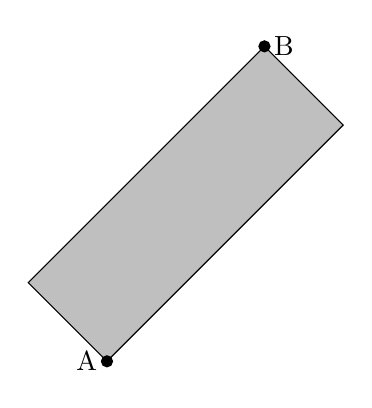
\begin{tikzpicture}
\fill [fill=lightgray] (0,0) -- (-1,1) -- (2,4) -- (3,3) -- cycle;
\draw  [latex-latex](0,0) -- (-1,1) -- (2,4)-- (3,3) -- cycle;

\filldraw (0,0) node[left] {A} circle (2pt);
\filldraw (2,4) node[right]{B} circle (2pt);
\end{tikzpicture}
\end{center}

Drop an altitude from B to line up horizontally with A and label the end-point D.
The length |AD| and |BD| are the coordinates.

\begin{center}
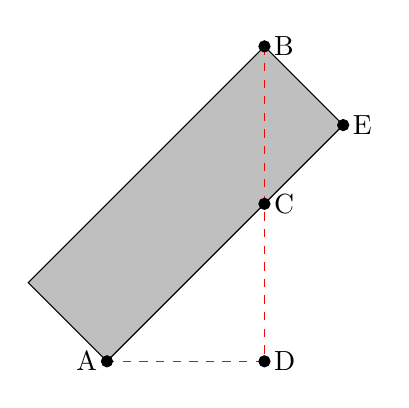
\begin{tikzpicture}
\fill [fill=lightgray] (0,0) -- (-1,1) -- (2,4) -- (3,3) -- cycle;
\draw  [latex-latex](0,0) -- (-1,1) -- (2,4)-- (3,3) -- cycle;

\draw[dashed,red] (2,4)-- (2,2)--(2,0) -- (0,0);

\filldraw (0,0) node[left] {A} circle (2pt);
\filldraw (2,4) node[right]{B} circle (2pt);
\filldraw (2,2) node[right]{C} circle (2pt);
\filldraw (2,0) node[right]{D} circle (2pt);
\filldraw (3,3) node[right]{E} circle (2pt);
\end{tikzpicture}
\end{center}

The triangles $\triangle$ACD and $\triangle$BCE are $45^\circ-90^\circ-45^\circ$ triangles meaning:
\begin{equation*}
\begin{aligned}
	\uline{AC} =& \sqrt{2}\uline{AD} \\
	\uline{BE} =& \frac{1}{\sqrt{2}}\uline{BC} \\
	=& \frac{1}{\sqrt{2}}(\uline{BD}-\uline{CD}) \\
	=& \frac{1}{\sqrt{2}}(\uline{BD}-\uline{AD}) \\
\end{aligned}
\end{equation*}

Hence the (signed) area of the rectangle is:
\begin{equation*}
\begin{aligned}
	\uline{BE}\cdot\uline{AE} =&\uline{BE}\cdot(\uline{AC}+\uline{CE}) \\
	=&(\uline{BD}-\uline{AD})(\uline{BD}+\uline{AD})\\
	=&\uline{BD}^2-\uline{AD}^2\\
\end{aligned}
\end{equation*}

\subsection{Causal Metric}
This construction supplies some intuition for Minkowski Metric.
Since if we interpret the plane as the set of events where the horizontal component is space-like and the vertical is time-like.
The reason the rectangle is at a $45^\circ$ is because that's the maximum speed of propagation.
The rectangle's area is a measure of the amount of events in-between the two.
And the sign of the area is the type of causal connection.
Wether the points are in the way (space-like), or another events are a means by which the earlier effect the later (time-like).

\let\uline\undefined

% Copyright 2023 Kieran W Harvie. All rights reserved.

\section{Quick Summary of Spaces}
A space is a collection of elements, often called points,
with some additional structure.
There are four main types of spaces that form a nice hierarchy,
that is that some types of spaces are always a subtype of other space.
\subsection{Hierarchy}
{\textbf{Topological Space: Neighbourhood}}
In a topological space the elements have a concept of "Neighbourhood",
that is the points which are adjacent to each point.
\begin{center}
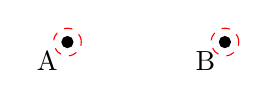
\begin{tikzpicture}
	\draw[dashed,red] (0,0) circle (5pt); 
	\filldraw (0,0) node[below left] {A} circle (2pt);
	\draw[dashed,red] (2,0) circle (5pt); 
	\filldraw (2,0) node[below left] {B} circle (2pt);
\end{tikzpicture}
\end{center}

{\textbf{Metric Space: Distance}}
In a metric space the element have a concept of distance to each other.
You can induce a neighbourhood by saying all points within a certain threshold distance to a point are in the neighbourhood of that point.
\begin{center}
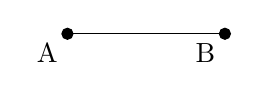
\begin{tikzpicture}
	\draw (0,0) -- (2,0);
	\filldraw (0,0) node[below left] {A} circle (2pt);
	\filldraw (2,0) node[below left] {B} circle (2pt);
\end{tikzpicture}
\end{center}

{\textbf{Normed Space: Length}}
In a normed space there is a concept of length of a point.
Shown here as their distance to some origin.
A distance can be induced by getting the length of an arrow going from A to B.
\begin{center}
\begin{tikzpicture}
	\draw[->] (0,0) -- (0,3.8);
	\draw[->] (0,0) -- (1.9,2.9);
	\filldraw (0,0) node[below] {O} circle (2pt);
	\filldraw (0,4) node[left] {A} circle (2pt);
	\filldraw (2,3) node[right] {B} circle (2pt);
\end{tikzpicture}
\end{center}


{\textbf{Inner-product Space: Projection}}
An inner product space has a concept of projecting one element on another.
You can induce a length by projecting an object onto itself.
\begin{center}
\begin{tikzpicture}
	\draw[->] (0,0) --(0,4.8);
	\draw[->] (0,0) -- (1.9,1.9);
	\draw[red,dashed] (2,2) -- (0,4);
	\draw (1.7,2.3) -- (1.4,2) -- (1.7,1.7);
	\filldraw (0,0) node[below] {O} circle (2pt);
	\filldraw (0,5) node[left] {A} circle (2pt);
	\filldraw (2,2) node[right] {B} circle (2pt);
	\filldraw (0,4) node[left] {B$'$} circle (2pt);
\end{tikzpicture}
\end{center}

\subsection{Euclidean}
Euclidean space is a normed space on $\mathbb{R}^n$ where the inner product is given by $\sum_k A_kB_k$.
This naturally induces a metric on $\mathbb{R}^n$.

The reason we care about the metric of Euclidean space is because all normed spaces have a form of the Pythagorean theorem.
Making metric space the most endowed space we can easily start thinking about non-Euclidean space.

This sucks because most talk about non-Euclidean space talks about "parallel lines" which makes one naturally think about angles and hence an inner product.
But no, instead we have the concept of a geodesic.
A geodesic is a curve that is locally distance minimizing.
This locality comes from the topology, and means that for all points $\gamma(t_1)$ and $\gamma(t_0)$ on the curve $\gamma$ such that they are in the same neighbourhood satisfy:
\[ d(\gamma(t_1),\gamma(t_0)) = k|t_1-t_2|\]

\subsection{non-Euclidean}
Quick rundown of some attempts of non-Euclidean geometries:

Pseudo-Euclidean: Like how we defined Euclidean Space was defined with an inner product we define a new structure with a different quadratic form.
\\

Riemann Manifold: A Manifold is a space that is "locally Euclidean". And a Riemann Manifold is one where this inner-product in the local Euclidean space is always positive.\\

Pseudo-Riemann Manifold: Like A Riemann Manifold but the inner-product is only required to be non-degenerate. I think this includes Pseudo-Euclidean space, but haven't put much thought into it.

%\documentclass[12pt]{article}
%\usepackage{amsmath}
%\usepackage{amssymb}

\section{Wave Equation}
\subsection{Symmetry}
Given some function $u(\vec{x},t)$ on space and time we want to understand it's dynamics under the following assumptions:
\begin{enumerate}
	\item {\textbf{Reversible}}, the dynamics should be symmetric in respect to reversing time.
	\item {\textbf{Isotropic}}, the function should be symmetric in respect to all directions.
	\item {\textbf{Relative}}, the absolute value doesn't matter, only changes.
	\item {\textbf{Perturbation}}, the changes should be small.
\end{enumerate}

The wave equation is a natural conclusion from from these constraints:
\[\frac{\partial^2}{\partial t^2}u = c\sum_i \frac{\partial^2}{\partial x_i^2} u\]

Because the change change is small we start by considering a Taylor expansion and try to get the lowest order terms.
Because it's relative we ignore the $0^\text{th}$ order terms.
Because it's reversible we ignore the $1^\text{st}$ order terms
Giving:
\[\frac{\partial^2}{\partial t^2}u = \sum_{i,j} w_{i,j}\frac{\partial^2}{\partial x_i \partial x_j} u\]
Because it's isotropic all the $\frac{\partial^2}{\partial x_i^2}$ coefficient need to be equal.
And without loss of generality we can assume a basis where the cross terms vanish, giving:
\[\frac{\partial^2}{\partial t^2}u = \sum_i cu\frac{\partial^2}{\partial x_i^2} = c\sum_i \frac{\partial^2}{\partial x_i^2} u\quad \square\]

\subsection{Old Symmetry Attempt}
(Not sure what I was doing here, lol. Seems like I went on the wrong path by not including $t$)
Lets start with with a function of space $u(\vec{x})$.
Lets assume it is continuous such that:
\[u(\vec{x} +\vec{r}) = u(\vec{x}) + \sum_{i}r_i\frac{\partial}{\partial x_i}u(\vec{x})+\frac{1}{2}\sum_{i,j}r_ir_j\frac{\partial^2}{\partial x_i\partial x_j}u(\vec{x}) \]
Lets remove all terms that aren't reversible:
\[u(\vec{x} +\vec{r}) = u(\vec{x}) + \frac{1}{2}\sum_{i}r_i^2\frac{\partial^2}{\partial x_i^2}u(\vec{x}) \]
Lets impose localization:
\[c^2r_0^2 = \sum_{i>0}r_i^2\]
Not sure exactly how this part works but we get the sign we need one example is to only keep terms that have $c^2r_0^2 = r_i^2$

\subsection{1-D}
I need to remind myself how to solve the 1-D case as a stepping stone for something else.
Reminder that the 1-D form, with unitary speed, is:
\[ \frac{\partial^2}{\partial t^2} u = \frac{\partial^2}{\partial x^2}u\]
Observe that plane waves where angular frequency and wave number have the same magnitude solve this:
\[ \exp(ik(x\pm t))\]
This suggests the use of Fourier transform, where the $\pm$ is used to fit the solution to initial value and derivative:
\[ u = \frac{1}{\sqrt{2\pi}}\int_\mathbb{R}(a_+(k)e^{ikt}+a_-(k)-e^{-ikt})e^{ikx}\,dk\]
Assume $f(x) = u(x,0)$ and $h(x) = \left[\frac{\partial}{\partial t}u\right](x,0)$.
Equating Fourier transforms gives:
\begin{equation*}
\begin{aligned}
	\hat{f}(k) =& a_+(k)+a_-(k) \\
	\hat{h}(k) =& ik(a_+(k)-a_-(k)) \\
\end{aligned}
\end{equation*}
Hence:
\[ u = \frac{1}{\sqrt{2\pi}}\int_\mathbb{R}(\hat{f}(k)\cos(kt)+\hat{h}(k)k^{-1}\sin(kt))e^{ikx}\,dk\]
\\

This can be processed further through the convolutions theorem.
(Because of the table of transforms I have it will be easier $\sin$ is turned into normalized $\sinc$ first):
\[ u = \frac{1}{\sqrt{2\pi}}\int_\mathbb{R}\left(\hat{f}(k)\cos(kt)+\hat{h}(k)t\sinc\left(\frac{kt}{\pi}\right)\right)e^{ikx}\,dk\]

\begin{equation*}
\begin{aligned}
	u =& \left[f(\tau)\ast\frac{1}{2}(\delta(\tau-t)+\delta(\tau+t))\right](x) + \frac{|t|}{2}\left[h(\tau)\ast\rect\left(\frac{\tau}{2t}\right)\right](x)\\
	 =&  \frac{1}{2}(f(x-t)+f(x+t)) + \frac{|t|}{2}\left[h(\tau)\ast\rect\left(\frac{\tau}{2t}\right)\right](x)\\
\end{aligned}
\end{equation*}

Which is such a cool equation!
It shows the reversibility and isotropic nature of the solution but the evenness of $x$ and $t$.
It shows the limit on how fast information travels by the convolution with $\rect$.

\section{Unit Fraction}
\textbf{Theorem:}
Consider a function $f:X \rightarrow \mathbb{R}$ where $\cl(\im(f))$ is bounded and countable.
Then for any $n\in\mathbb{N}$ and interval $U\subset \mathbb{R}$ we have $n\im(f) \not\supseteq\mathbb{Q} \cap U$.
\footnote{In this section $nS$ means $\{\sum_i s_i | s\in S^n\}$ and not $\{ns | s\in S\}$} 
\\

\textbf{Proof:}
If we assume that $n\im(f) \supseteq \mathbb{Q} \cap U$ we get:
\[|\cl(n\im(f))| \geq |\cl(\mathbb{Q} \cap U)| = |U| = \aleph_1 \]
However by the compactness of $\cl(\im(f))$:
\[\cl(n\im(f))= n\cl(\im(f))\]
Hence by the countability of $\cl(\im(f))$:
\[|\cl(n\im(f))| = |n \cl(\im(f))| \leq |\cl(\im(f))|^n = \aleph_0^n = \aleph_0\]
This contradicts $|\cl(n\im(f))| \geq \aleph_1$ and hence $n\im(f) \not\supseteq\mathbb{Q} \cap U$.
\\

\textbf{Corollary:}
The function $f:\mathbb{N}_{>0} \rightarrow \mathbb{R}$ where $f(x) = 1/x$ meets the function requirements.
Hence for every interval there is a rational number that can't be represented with $n$ unit fractions.
\\

I want to try a more aesthetically pleasing formulation by separating out the set theory from the topology from the $\mathbb{Q}$ specifics. 
\\

\textbf{Theorem:} Let $X$ and $Y$ be sets. 
Then $|Y| > |X|^n$ implies $nX \not\supseteq Y$.

\textbf{Proof:} By contradiction on set size.
\\

\textbf{Theorem:} If $X$ is countable and $Y$ is non-countable then $nX \not\supseteq Y$ for all $n\in\mathbb{N}_{>0}$.

\textbf{Proof:} The previous theorem using $\aleph_1 > \aleph_0^n$ for all $n\in\mathbb{N}_{>0}$
\\

\textbf{Theorem:} If $X$ is compact, $\cl(X)$ countable, and $Y$ non-countable then $\cl(nX) \not\supseteq Y$ for all $n\in\mathbb{N}_{>0}$.

\textbf{Proof:} The previous theorem using $\cl(nX) = n\cl(X)$ from compactness.
\\

Now just rework the corollary a bit for it to fit here. 

\section{Winquist's identity}
The following form of the Winquist's identity was on an old hard drive:
\begin{equation*}
\begin{aligned}
	\prod_{n \geq 1}&(1-ax^{n-1})(1-a^{-1}x^n)(1-bx^{n-1})(1-b^{-1}x^{n}) \\
	&\times(1-ab^{-1}x^{n-1})(1-abx^{n-1})(1-a^{-1}b^{-1}x^{n})(1-x^n)^2 \\
	=& \sum_{i \in \mathbb{N}_{\geq 0}}\sum_{j\in\mathbb{Z}} (-1)^{i+j}(b^{-3j}-b^{3j+1})(a^{-3i}-a^{3i+3}) \\
	&\times(b^{-3i+2}-b^{3i-1})(a^{-3j+1}-a^{3j+2})x^{\frac{j(3j+1)}{2}+\frac{3i(i+1)}{2}} \\
\end{aligned}
\end{equation*}

A quick Google make the identity verifies that the identity looks right.
With the exception of the ranges of the RHS summation, maybe $i$ and $j$ should be switched.
\\

Either way this is a cool identity and captures something interesting.
And that would definitely be helpful in generating functions.
In particular reciprocating the relation and multiplying by the RHS give a weighted partition that has a relatively sparse recursive relation.

% Copyright 2023 Kieran W Harvie. All rights reserved.

\section{XOR hash}
Today I was presented with the following problem:
\\

Given an array with all integers $[1,100]$ with a single integer removed.
Assuming memory is limited, how do you efficiently determine the missing integer?
\\

The solution is to XOR all the elements of the array together.
Then XOR this with the known value for ALL the numbers between $[1,100]$.
The result will be the missing number.
\\

This problem seemed like a good introduction to hashes, like Zobrist, that XOR a bunch of info together.
The benefit of this approach is that the components can be added/removed by a XOR:
\[h(\{a_0,a_1\}) = h(\{a_0\})\text{ XOR }h(\{a_1\})\]

\subsection{Determining the constant}
It turns out its easy to calculate the constant for the original question by hand.
First define $T$ as:
\[T(n) = n \text{ XOR } T(n-1),\quad T(1) = 1\]
Then:
\[T(n) = \begin{cases}n&n \mod 4 = 0 \\1& n\mod 4 = 1\\ n+1 &n\mod 4 = 2\\ 0& n\mod 4 = 3\end{cases}\]
This can easily be proved by induction and remembering that for even $n$ we have:
\[n\text{ XOR } 1 = n+1\]

Because of the modularity you would expect there to be an expression for $T$ involving powers of the fourth root of unity ($i$): 
\[T(n) = \frac{1}{2} +\frac{1}{2}(1+(-1)^n)+\frac{1}{4}((i-1)(-i)^n-(i+1)i^n)\]
(Done on scrap paper, not double checked, close enough to see the form).
\\

While the hybrid function is probably a more useful form the last one involves complex numbers in a way I didn't expect.

% Copyright 2023 Kieran W Harvie. All rights reserved.
\section{Rational Tangent}
Consider the following relation:
\begin{equation*}
\begin{aligned}
	\cos(n\phi)+i\sin(n\phi) =& (\cos(\phi)+i\sin(\phi))^{n} \\
	=&(\cos(\phi)(1+i\tan(\phi)))^n\\
	=&\cos(\phi)^n(1+i\tan(\phi))^n\\			
\end{aligned}
\end{equation*}
The product of two complex numbers with rational real and imaginary part is a complex number with rational real and imaginary part.

To see this observe that we only use multiplication, addition, and subtraction to get the real and imaginary components of the product from the component of the factors and that these operations between from rational numbers produce rational numbers.

Hence, if $\tan(\phi)$ is rational the there exists some rational numbers $p,q$ such that:
\[(1+i\tan(\phi))^n = p+qi\]
Substituting this into the original formula:
\[\cos(n\phi)+i\sin(n\phi) = \cos(\phi)^n(p+qi)\]
And equating real and imaginary components gives:
\[\tan(n\phi) = \frac{\sin(n\phi)}{\cos(n\phi)} = \frac{\cos(\phi)^np}{\cos(\phi)^nq} = \frac{p}{q}\]

Hence $\tan(\phi)$ being rational implies $\tan(n\phi)$ is as well.
\\

I think this result was meant to be part of a larger argument,
but I have forgotten what the larger one is.
One point that I think will be relevant is using similar arguments with:
\[\frac{1}{\cos(\phi)+i\sin(\phi)}= \cos(\phi)-i\sin(\phi)\]

\subsection{Brute Force}
Another proof of the same result, 
done by brute force,
was in the same notes on my hard-drive.
Presumably done as a sanity check before figuring out the better method:
\\

$\tan(\phi)$ being rational is the same as saying that $r\sin(\phi) = \cos(\phi)$ for some rational number $r$.
\begin{equation*}
\begin{aligned}
	\sin(n\phi)+i\cos(n\phi) =& \exp(in\phi)\\
	=& \exp(i\phi)^n \\
	=& (\sin(\phi)+i\cos(\phi))^n\\
	=& \sum_{k=0}^{n}\binom{n}{k}i^k\cos(\phi)^k\sin(\phi)^{n-k}\\
	=& \sum_{k=0}^{n}\binom{n}{k}i^kr^k\sin(\phi)^n\\
	=&\sin(\phi)^n\left(\sum_{k=0}^{2k \leq n}\binom{n}{2k}(-1)^kr^{2k}+i\sum_{k=0}^{2k+1 \leq n}\binom{n}{2m+1}(-1)^kr^{2k+1}\right)\\
\end{aligned}
\end{equation*}
Hence:
\[\tan(n\phi) = \frac{\sum_{k=0}^{2k \leq n}\binom{n}{2k}(-1)^kr^{2k}}{\sum_{k=0}^{2k+1 \leq n}\binom{n}{2k+1}(-1)^kr^{2k+1}}\]


% Copyright 2023 Kieran W Harvie. All rights reserved.

\section{Jensen's Inequality}
A convex function $\phi$ on a set $X$ is one such that for $a_n\in X$ with $w_0+w_1 =1$ and $w_n \geq 0$ then we have:
\[\phi(w_0a_0+w_1a_1) \leq w_0\phi(a_0)+w_1\phi(a_1)\]
Jensen's Inequality states that expected value of the function is less then the function of the expected value:
\[\phi(\E(X)) \leq \E(\phi(X))\]

By multiplying the function by $-1$, we get the intuitive corollary that the inequality is reversed for concave functions.

\subsection{Generalization}
A more general form of convexity can be easily proved by induction.
\\

Assume that for some $n$ we have that for all $\sum_{i=1}^nw_i'=1$ and $w_i' \geq 0$:
\[\phi\left(\sum_{i=1}^nw_i'a_i\right) \leq \sum_{i=1}^nw_i'\phi(a_i)\]

Let $\sum_{i=1}^{n+1}w_i=1$ and $W = \sum_{i=1}^nw_i$ we have $w_{n+1}+W = 1$ and :
\begin{equation*}
\begin{aligned}
\phi\left(\sum_{i=1}^{n+1}w_ia_i\right) =&\phi\left(w_{n+1}a_{n+1}+W\sum_{i=1}^{n}\frac{w_i}{W}a_i\right) \\
\leq& w_{n+1}\phi(a_{n+1})+W\phi\left(\sum_{i=1}^{n}\frac{w_i}{W}a_i\right) \\
\leq& w_{n+1}\phi(a_{n+1})+W\sum_{i=1}^n\frac{w_i}{W}\phi(a_i) \\
\leq& \sum_{i=1}^{n+1}w_i\phi(a_i) \\
\end{aligned}
\end{equation*}

Viewing the weights as probabilities this form can directly be in interpreted as a discrete form of Jensen's Inequality.

\subsection{Mean Inequalities}
This can be directly applied to various mean inequalities.
\begin{equation*}
\begin{aligned}
	AM =& \frac{1}{n}\sum_{i=1}^{n}a_i \\
	RMS =& \sqrt{\frac{1}{n}\sum_{i=1}^na_i^2} \\
	GM =& \sqrt[n]{\prod_{i=1}^na_i}\\
\end{aligned}
\end{equation*}
Using $\phi(x)=x^2$,$w_i = \frac{1}{n}$ we directly get:
\[AM^2 \leq RMS^2\]
Using $\phi(x)=\log(x)$,$w_i = \frac{1}{n}$ we get:
\footnote{Remember that the inequality is reversed since $\log$ is concave}
\[\log(AM) \geq \log(GM)\]

Since both these functions are also monotonic the clean relations follow.

\subsection{Decision Theory} 
Interpret $\phi$ as a utility function then the convexity tells us whether we take the fixed $\E(X)$ or risk $X$.
Well if $\phi$ is convex then:
\[\phi(\E(X)) \leq \E(\phi(X))\]
And we should take the risk,
there is more expected utility taking the risk then the utility of $\E(X)$.

If $\phi$ is concave then we should not take the risk.

% Copyright 2023 Kieran W Harvie. All rights reserved.

\section{Convex}
TODO: Flesh out, copy edit, and maybe include pictures for the geometric intuition in the cord section.
\\

In the section of Jensen's Inequality I defined a convex function $\phi$ on a set $X$ as one such that for $a_n\in X$ with $w_0+w_1 =1$ and $w_n \geq 0$ then we have:
\[\phi(w_0a_0+w_1a_1) \leq w_0\phi(a_0)+w_1\phi(a_1)\]
I've thought of another proof of the previous section but iterates over functions instead of points.
And we can use some geometry intuition (cords).
\\

\subsection{Cords}
First let me define a new function called the cord function that takes on an interval $[a,b] \subseteq X$:
\[C_{[a,b]}(x) = \phi(a)+(x-a)\frac{\phi(b)-\phi(a)}{b-a}\]
The convex property can be changed to:
\[x\in [a,b] \Rightarrow \phi(x) \leq C_{[a,b]}(x)\]

{\bf Lemma:}, if $x_0 \leq x_1 \leq x_2$ then:
\[ x\in [x_0,x_1] \Rightarrow C_{[x_0,x_1]}(x) \leq C_{[x_0,x_2]}(x)\]
and:
\[ x\in [x_1,x_2] \Rightarrow C_{[x_1,x_2]}(x) \leq C_{[x_0,x_2]}(x)\]
{\bf Proof:} Use $C_{[a,b]}(a) = \phi(a)$ or $C_{[a,b]}(b) = \phi(b)$ and $x_1 \in [x_0,x_2]$ with the definition of convexity.
\\

{\bf Lemma:}, if $a_0 \leq a_1 \leq b_1 \leq b_0$ then:
\[x\in [a_1,b_1] \Rightarrow C_{[a_1,b_1]}(x) \leq C_{[a_0,b_0]}(x)\]
{\bf Proof:} use the previous lemma with the triples form the quad inequality, then chain together the newer inequalities.
\\

Let:
\[\phi_{[A,B]}(x) = \begin{cases} C_{[A,B]}(x) & x\in [A,B] \\ \phi(x) &\text{else} \end{cases}\]
$\phi_{[A,B]}(x)$ is convex.
Prove this using the previous lemmas with the three cases (points same side, both sides, one in one out).

\subsection{The Cool Proof}
We want to show that for all $\sum_{i=1}^nw_i'=1$ and $w_i' \geq 0$:
\[\phi\left(\sum_{i=1}^nw_i'a_i\right) \leq \sum_{i=1}^nw_i'\phi(a_i)\]

Assume it works for $n-1$ points.
Take two points $(w_0,a_0)$ and $(w_1,a_1)$ and make a new convex function using the method from the previous section with $[x_0,x_1]$, then remove the two points and replace with $(w_0+w_1, \frac{w_0a_1+w_1a_1}{w_1+w_0})$.
Now we have a $n-1$ points,
and if you expand the algebra you get the correct form,
hence by induction you prove the initial result.

% Copyright 2023 Kieran W Harvie. All rights reserved.
\section{Old Geometry}
Bellow are are collection of proofs from high school that I saved under "geometry".
It includes triangle groups and two (half complete) geodesics.
\subsection{Triangle Groups}
Are a way of understanding the rotations of platonic solids.
Fill in latter
\subsubsection{Subgroup chain}
Let:
\[\iota^2 = \lambda^4 = \kappa^3 = 1\]
With and those be the lowest powers that do so.
Additionally have:
\[\lambda = \iota\kappa\]
This is a cube, $\iota$ rotates around a edge, $\kappa$ rotates around a vertex, $\lambda$ rotates around a face.

Let:
\[i = \lambda^2,\,k=\lambda\iota,\,k=\kappa^2\]
We have:
\begin{equation*}
\begin{aligned}
i^2 =& \lambda^4\\
	=& 1 \\
k^3 =& \kappa^6\\
	=&1\\
l^3 =& (\lambda\iota)^3\\
	=&(\iota\kappa\iota)^3\\
	=&\iota\kappa^3\iota\\
	=&1\\
\end{aligned}
\end{equation*}
These are the lowest powers to do so.
Minimality is trivial for $i$ and $k$ by the minimality of $\kappa$ and $\iota$.
For $l$ assume $l^2 = 1$ then:
\begin{equation*}
\begin{aligned}
l^2 =& 1\\
\lambda\iota\lambda\iota =& 1\\
\iota\lambda\iota =& \lambda^3\\
\kappa\iota =& \lambda^3\\
\kappa\iota\lambda =& \lambda^4\\
=&1\\
\kappa^2 =& 1\\
\end{aligned}
\end{equation*}
We have the relation:
\begin{equation*}
\begin{aligned}
ik =& \lambda^3\iota\\
	=&\lambda^3\iota\kappa^3\\
	=&\lambda^3\lambda\kappa^2\\
	=&\kappa^2\\
\end{aligned}
\end{equation*}
Hence the rotations of a regular tetrahedron are a subgroup of the rotations of a cube.
\subsection{Torus}
Let a torus be parametrized by:
\begin{equation*}
\begin{aligned}
	r =&\,(x,y,z) \\
	x =&\, (R+r\cos(\theta))\cos(\phi)\\
	y =&\, (R+r\cos(\theta))\sin(\phi)\\
	z =&\, r\sin(\theta) \\
\end{aligned}
\end{equation*}
The partials of r are given by:
\begin{equation*}
\begin{aligned}
	\frac{\partial r}{\partial \phi} =&\, (-(R+r\cos(\theta))\sin(\phi),(R+r\cos(\theta))\cos(\phi),0) \\
	\frac{\partial r}{\partial \theta} =&\, (-r\sin(\theta)\cos(\phi),-r\sin(\theta)\sin(\phi),r\cos(\theta)) \\
	\frac{\partial r}{\partial \phi}\cdot\frac{\partial r}{\partial \phi} =&\, (R+r\cos(\theta))^2 \\
	\frac{\partial r}{\partial \theta}\cdot\frac{\partial r}{\partial \theta} =&\, r^2 \\
	\frac{\partial r}{\partial \theta}\cdot\frac{\partial r}{\partial \phi} =&\, 0 \\
\end{aligned}
\end{equation*}
Use the partial to get the line element:
\begin{equation*}
\begin{aligned}
	\dot{r}^2 =&\, \left(\frac{\partial r}{\partial \phi}\dot{\phi} + \frac{\partial r}{\partial \theta}\dot{\theta}\right)^2 \\
	=&\, \frac{\partial r}{\partial \phi}\cdot\frac{\partial r}{\partial \phi}\dot{\phi}^2+ \frac{\partial r}{\partial \theta}\cdot\frac{\partial r}{\partial \theta}\dot{\theta}^2+2\frac{\partial r}{\partial \theta}\cdot\frac{\partial r}{\partial \phi} \dot{\phi}\dot{\theta} \\
	=&\, (R+r\cos(\theta))^2\dot{\phi}^2+ r^2\dot{\theta}^2\\
\end{aligned}
\end{equation*}
Treating the line element as the integrand in Lagrangian integral:
\[ L = \frac{1}{2}\dot{r}^2\]
\begin{equation*}
\begin{aligned}
	\frac{\partial L}{\partial \phi} =& \frac{d}{d t}\frac{\partial L}{\partial \dot{\phi}}\\	
	0 =& \frac{d}{d t}(R+r\cos(\theta))^2\dot{\phi} \\
	=& \left[\dot{\theta}\frac{\partial}{\partial \theta} + \ddot{\phi}\frac{\partial}{\partial \dot{\phi}}\right](R+r\cos(\theta))^2\dot{\phi} \\
	=& (R+r\cos(\theta))^2\ddot{\phi}-2r\sin(\theta)(R+r\cos(\theta))\dot{\phi}\dot{\theta} \\
	\ddot{\phi} =& \frac{2r\sin(\theta)}{R+r\cos(\theta)}\dot{\phi}\dot{\theta} \\
\end{aligned}
\end{equation*}
And again:
\begin{equation*}
\begin{aligned}
	\frac{\partial L}{\partial \theta} =& \frac{d}{d t}\frac{\partial L}{\partial \dot{\theta}}\\	
	-r\sin(\theta)(R+r\cos(\theta))\ddot{\phi}^2 =& r^2\frac{d}{dt}\dot{\theta} \\
	-r\sin(\theta)(R+r\cos(\theta))\ddot{\phi}^2 =& r^2\ddot{\theta} \\
\end{aligned}
\end{equation*}
\subsection{Sphere}
Let a sphere be parametrized by:
\begin{equation*}
\begin{aligned}
	r =&\,(x,y,z) \\
	x =&\, \cos(\theta)\cos(\phi)\\
	y =&\, \cos(\theta)\sin(\phi)\\
	z =&\, \sin(\theta) \\
\end{aligned}
\end{equation*}
The partials of r are given by:
\begin{equation*}
\begin{aligned}
	\frac{\partial r}{\partial \phi} =&\,(-\cos(\theta)\sin(\phi),\cos(\theta)\cos(\phi),0)\\
	\frac{\partial r}{\partial \theta} =&\, (-\sin(\theta)\cos(\phi),-\sin(\theta)\sin(\phi),\cos(\theta)) \\
	\frac{\partial r}{\partial \phi}\cdot\frac{\partial r}{\partial \phi} =&\, \cos(\theta)^2 \\
	\frac{\partial r}{\partial \theta}\cdot\frac{\partial r}{\partial \theta} =&\, 1 \\
	\frac{\partial r}{\partial \theta}\cdot\frac{\partial r}{\partial \phi} =&\, 0 \\
\end{aligned}
\end{equation*}
Use the partial to get the line element:
\begin{equation*}
\begin{aligned}
	\dot{r}^2 =&\, \left(\frac{\partial r}{\partial \phi}\dot{\phi} + \frac{\partial r}{\partial \theta}\dot{\theta}\right)^2 \\
	=&\, \frac{\partial r}{\partial \phi}\cdot\frac{\partial r}{\partial \phi}\dot{\phi}^2+ \frac{\partial r}{\partial \theta}\cdot\frac{\partial r}{\partial \theta}\dot{\theta}^2+2\frac{\partial r}{\partial \theta}\cdot\frac{\partial r}{\partial \phi} \dot{\phi}\dot{\theta} \\
	=&\, \cos(\theta)^2\dot{\phi}^2+ \dot{\theta}^2\\
\end{aligned}
\end{equation*}
Geodesic Equations:
\begin{equation*}
\begin{aligned}
	\ddot{\theta} =& -\sin(\theta)\cos(\theta)\dot{\phi}^2\\
	0 =& \frac{d}{dt}\cos(\theta)^2\dot{\phi} \\
	=& \cos(\theta)^2\ddot{\phi}-2\cos(\theta)\sin(\theta)\dot{\phi}\dot{\theta} \\
\end{aligned}
\end{equation*}
Consider the function:
\begin{equation*}
\begin{aligned}
	f(t) =& z + \alpha x + \beta y \\
	f(t) =& \sin(\theta) + \alpha\cos(\theta)\cos(\phi) + \beta\cos(\theta)\sin(\phi) \\
	\dot{f}(t) =& \dot{\theta}\cos(\theta)+\alpha(-\dot{\theta}\sin(\theta)\cos(\phi)-\dot{\phi}\cos(\theta)\sin(\phi)) + \beta(-\dot{\theta}\sin(\theta)\sin(\phi)+\dot{\phi}\cos(\theta)\cos(\phi))\\
\end{aligned}
\end{equation*}

\begin{equation*}
\begin{aligned}
\end{aligned}
\end{equation*}


\end{document}
